\cleardoublepage

\chapter{LoRaWAN}


\begin{wrapfigure}{r}{4cm}

\includegraphics[width=.3\columnwidth]{Pictures/LORAWAN-logo.png}
\end{wrapfigure}


\lgf{Avec \Index{Sigfox}, ce n’était que du bonheur ! Nous avions un environnement unique développé par un seul acteur. L’attachement d’un objet au réseau, la récupération des données s’en trouve grandement simplifiée.}
\lge{With \Index{Sigfox}, it was only happiness! We had a unique environment developed by a single actor. Attaching an object to the network, retrieving data was greatly simplified.}


\lgf{Avec \Index{LoRaWAN}, l'écosystème est plus complexe. Pour rappel, \Index{LoRa} est une modulation longue portée et LoRaWAN un protocole de niveau 2 qui a pour but de fédérer les acteurs (fabricants d’objets, utilisateurs d’objets, opérateur de réseaux) autour de la communication radio entre l’objet et le cœur de réseau appelé ici \ac{LNS} . Mais l’enregistrement des objets, le lien entre les applications et le LNS diffèrent d’un réseau à un autre.}
\lge{With \Index{LoRaWAN}, the ecosystem is more complex. As a reminder, \Index{LoRa} is a long range modulation and LoRaWAN is a level 2 protocol which aims to federate the actors (object manufacturers, object users, network operators) around the radio communication between the object and the network core called here \ac{LNS} . But the registration of objects, the link between applications and the LNS differ from one network to another.}


     \vspace{1em}

\lgf{Même si vous n’avez pas l’intention de mettre en œuvre le réseau Sigfox, nous vous recommandons de lire le chapitre précédent (ou à la rigueur de le survoler) car nous y ferons référence dans la suite du texte.}
\lge{Even if you do not intend to implement the Sigfox network, we recommend you to read the previous chapter (or at least to skim it) because we will refer to it in the following text.}

     \vspace{1em}

\lgf{LoRaWAN, comme Sigfox, opère dans la même bande de fréquences non licenciées. Il existe plusieurs opérateurs de réseaux LoRaWAN~:}
\lge{LoRaWAN, like Sigfox, operates in the same unlicensed frequency band. There are several LoRaWAN network operators:}

\begin{itemize}
    \item  
        \lgf{\ac{TTN}\footnote{\url{https://www.thethingsnetwork.org/}} propose une approche communautaire. Chaque personne peut mettre à disposition des passerelles radio pour la communauté et inscrire des objets. TTN gère le cœur de réseau. Si cette approche est sympathique, la couverture va être très parcellaire et va dépendre de la densité de geeks dans une région. De plus, la couverture du réseau va dépendre de la position des antennes qui doivent être placées sur un point haut. Avoir une antenne sur son balcon n’implique pas une grande couverture de la zone. Si vous avez de la chance, vous pourrez peut-être bénéficier d’un accès via TTN. Nous verrons comment s’y connecter.}
        \lge{\ac{TTN}\footnote{\url{https://www.thethingsnetwork.org/}} proposes a community approach. Each person can provide radio gateways for the community and register objects. TTN manages the core network. If this approach is nice, the coverage will be very patchy and will depend on the density of geeks in a region. Furthermore the coverage of the network will depend on the position of the antennas which must be placed on a high point. Having an antenna on your balcony does not imply great coverage of the area. If you are lucky, you may be able to get access via TTN. We will see how to connect to it.}
    \item   
        \lgf{des opérateurs nationaux comme, en France, \Index{Orange} ou \Index{Bouygues Télécom}. Mais il faut généralement bourse délier pour connecter les objets et pour limiter l’usage du downlink ; l’envoi des messages vers les capteurs est facturé en supplément. En revanche, la couverture est supérieure.}
        \lge{national operators such as, in France, \Index{Orange} or \Index{Bouygues Télécom}. But it is generally necessary to untie the purse to connect the objects and to limit the use of the downlink; the sending of messages to the sensors is charged extra. On the other hand, the coverage is superior.}
    \item   
        \lgf{les réseaux privés. Il est possible de faire tourner son propre LNS. Cela implique d’acheter des composants pour faire une passerelle radio. Mais il existe des mises en oeuvre ouvrete du LNS comme \Index{chirpstack}\footnote{\url{https://www.chirpstack.io/}}.} 
        \lge{private networks. It is possible to run your own LNS. It implies to buy components to make a radio gateway. But there are open implementations of LNS like \Index{chirpstack}\footnote{url{https://www.chirpstack.io/}}.} 
\end{itemize}

\lgf{\section{Information sur le LoPy}}
\lge{\section{Information about LoPy}}

\lgf{Chaque objet va avoir un identifiant unique codé sur 64 bits appelé \textit{\Index{devEUI}}. Cette information est nécessaire pour faire entrer un équipement sur le réseau. Le programme \lprog{lorawan\_devEUI.py}{pycom} donne accès à cette valeur qui est unique pour chaque LoPy.}
\lge{Each object will have a unique identifier coded on 64 bits called \textit{Index{devEUI}}. This information is necessary to enter a device on the network. The program \lprog{lorawan\_devEUI.py}{pycom} gives access to this value which is unique for each LoPy.}

\pycomlst{lorawan\_devEUI.py}\label{prog-devEUI}

\lgf{L’objet Python \pfunction{network}{LoRa} est importé du module \texttt{network} et une instance est créée ligne 5. La variable \texttt{mac} va stocker l’adresse MAC (autre nom du \textit{devEUI}) retournée par l’objet \texttt{lora} et l'afficher en hexadécimal, comme le montre l’exemple suivant~:}
\lge{The Python object \pfunction{network}{LoRa} is imported from the module \texttt{network} and an instance is created line 5. The variable \texttt{mac} will store the MAC address (another name for the \textit{devEUI}) returned by the \texttt{lora} object and display it in hexadecimal, as shown in the following example:}

\begin{termc}[backgroundcolor=\color{gray!10}, basicstyle=\ttfamily\small, escapechar=@] 
>>> Running lorawan_devEUI.py

>>>
>>>
devEUI:  b'70b3d54994c61237'
\end{termc}

\lgf{On a le \textit{devEUI}. Il manque encore 3 informations :}
\lge{We have the \textit{devEUI}. There are still 3 pieces of information missing:}

\begin{itemize}
    \item 
        \lgf{\textit{\Index{appEUI}} : c’est un identifiant sur 64 bits comme le \textit{devEUI} qui va servir à identifier l’application. On peut le mettre à 0~;}
        \lge{\textit{\Index{appEUI}}: it is an identifier on 64 bits like the \textit{devEUI} which will be used to identify the application. It can be set to 0;}
   \item 
        \lgf{\textit{\Index{AppKey}} : c’est une valeur sur 128 bits qui n’est connue que de l’objet et du LNS. Elle permet de dériver les clés de chiffrement utilisées par la suite ;}
        \lge{\textit{\Index{AppKey}} : it is a value on 128 bits which is known only by the object and the LNS. It allows to derive the encryption keys used afterwards;}

\end{itemize}

     \vspace{1em}

\lgf{Et sur le LNS, il faudra aussi configurer le connecteur~: il s’agit d’indiquer au LNS comment envoyer les données vers une application. Il peut s’agir de POST HTTP comme nous avons vu avec la configuration du \textit{\Index{backend}} avec Sigfox. Bien entendu, une fois ces grands principes établis, ça serait trop simple si tous les réseaux fonctionnaient de la même façon. Nous allons donc voir comment faire avec le réseau TTN. }
\lge{And on the LNS, it will also be necessary to configure the connector~: it is a question of indicating to the LNS how to send the data towards an application. It can be POST HTTP as we have seen with the configuration of the \textit{Index{backend}} with Sigfox. Of course, once these main principles are established, it would be too simple if all networks worked the same way. So we will see how to do with the TTN network. }


\section{The Things Network}


\begin{wrapfigure}{r}{3cm}
\Youtube{https://youtu.be/G69mjg80-mA}
\end{wrapfigure}

\lgf{The Things Network, ou TTN pour les intimes, est un réseau communautaire qui permet à tout un chacun de connecter soit une passerelle radio pour le bénéfice de la communauté, soit un objet. TTN se charge de faire tourner un LNS et de renvoyer les informations collectées à son propriétaire .On espère qu'un bon samaritain a déployé une antenne près de chez vous pour capter votre trafic. On n'a aucun moyen de savoir, si on n'essaye pas. }
\lge{The Things Network, or TTN for short, is a community network that allows anyone to connect either a radio gateway for the benefit of the community, or an object. TTN takes care of running an LNS and sending the collected information back to its owner. We hope that a good samaritan has deployed an antenna near you to pick up your traffic. We have no way of knowing, if we don't try. }


     \vspace{1em}

\lgf{La première étape consiste à se créer un compte, gratuit comme il se doit, sur le site de TTN~: \url{https://www.thethingsnetwork.org/}.}
\lge{The first step is to create an account, free as it should be, on the TTN~ website: \url{https://www.thethingsnetwork.org/}.}

     \vspace{1em}


\lgf{Une fois le formulaire de création de compte rempli et validé, vous disposez d’un accès au réseau TTN. 
Votre identifiant apparaît en haut à droite de la page Web. }
\lge{Once the account creation form has been completed and validated, you will have access to the TTN network. 
Your login appears in the top right corner of the web page. }

\begin{itemize}
    \item 
        \lgf{Cliquez sur votre nom,}
        \lge{Click on your name,}
    \item 
        \lgf{sélectionnez Console,}
        \lge{choose Console,}
    \item 
        \lgf{puis votre zone géographique (cela n'a rien à voir avec le plan de fréquence. Il est préférable de choisir le serveur le plus proche pour optimiser les communications).}
        \lge{then your geographical area (this has nothing to do with the frequency plan. It is better to choose the nearest server to optimize communications).}
\end{itemize}


\lgf{On peut soit définir une application et y associer des objets, soit connecter une passerelle radio (\textit{Go To Gateways}). Par la suite, nous explorerons cette option si vous voulez installer votre propre passerelle radio. Nous allons nous intéresser à la création d'application en choisissant \textit{Go To Applications}. TTN vous invite à créer notre première application ; cliquez sur le lien \textit{+Add Application}.}
\lge{You can either define an application and associate objects with it, or connect a radio gateway (\textit{Go To Gateways}). Later on, we will explore this option if you want to install your own radio gateway. We will focus on application creation by choosing \textit{Go To Applications}. TTN invites you to create our first application; click on the \textit{+Add Application} link.}


\lgf{\subsection*{Définir une application}}
\lge{\subsection*{Define an application}}

\lgf{Une application pour TTN va intégrer plusieurs objets LoRaWAN qui enverrons leur information à une application tournant sur un \ac{AS}. 
Il faut remplir le formulaire (cf. figure~\vref{fig-ttn-app}) en indiquant~:}
\lge{An application for TTN will integrate several LoRaWAN objects which will send their information to an application running on an AS. 
The form (see figure~\vref{fig-ttn-app}) must be filled in by indicating:}


\begin{itemize}
    \item 
        \lgf{l'identifiant de l'application. Il s'agit d'un nom uniquement composé de lettres et de chiffres ainsi que du tiret. Il doit être unique pour TTN. Donc, faites preuve d'imagination car il doit être unique pour TTN. Ce nom se retrouvera dans les URI permettant de piloter l'application ;}
        \lge{the application identifier. It is a name composed only of letters and numbers and a dash. It must be unique for TTN. So be creative because it must be unique for TTN. This name will be found in the URIs allowing to drive the application;}
    \item 
        \lgf{le nom de l'application qui apparaîtra dans les menus. Il n'y a pas de contraintes ; il vaut mieux choisir quelque chose d'explicite ;}
        \lge{the name of the application that will appear in the menus. There are no constraints; it is better to choose something explicit;}
    \item 
        \lgf{une description de l'application si nécessaire.}
        \lge{a description of the application if necessary.}
\end{itemize}

\begin{figure}[tbp]
\centerline{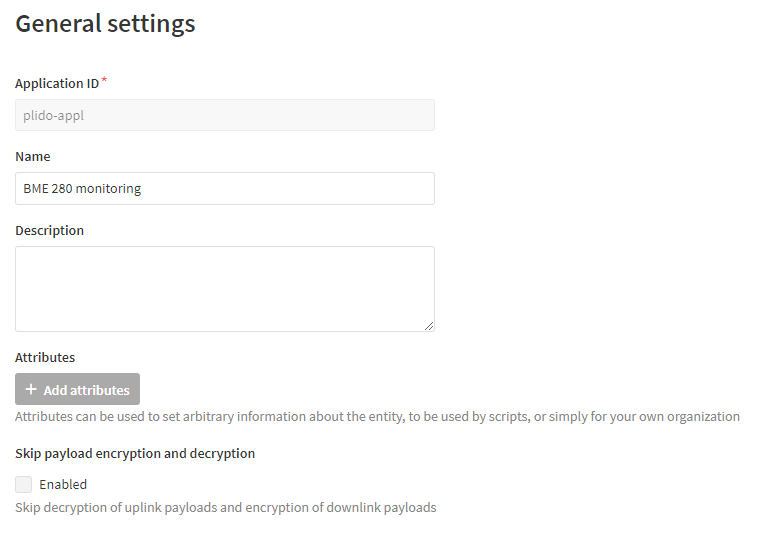
\includegraphics[width=0.7\columnwidth]{Pictures/ttn-app.png} }
\lgf{\caption{Configuration d'une application.}}
\lge{\caption{Configuration of an application.}}
\label{fig-ttn-app}
\end{figure}

     \vspace{1em}

\lgf{Cliquez sur Create Application pour enregistrer cette application. Vous arrivez sur un page de contrôle de votre application.}
\lge{Click on Create Application to register this application. You will be taken to a control page for your application.}


\lgf{\subsubsection*{Ajout d'un objet}}
\lge{\subsubsection*{Adding an object}}


\lgf{Nous devons enregistrer un ou plusieurs objets dans notre application~:}
\lge{We need to register one or more objects in our application:}

\begin{itemize}
    \item 
        \lgf{Cliquez sur \textit{end devices} dans le menu de gauche~;}
        \lge{Click on \textit{end devices} in the left menu;}
    \item 
        \lgf{puis \textit{+ Add end device}~;}
        \lge{puis \textit{+ Add end device};}
    \item 
        \lgf{et \textit{try manual registration} en dessous du menu déroulant. TTN offre des aides à la configuration pour certains objets, mais comme nous sommes des experts, nous n'en n'avons pas besoin.}
        \lge{and \textit{try manual registration} below the drop-down menu. TTN offers configuration aids for some objects, but since we are experts, we don't need them.}
\end{itemize}

     \vspace{1em}


\lgf{Le menu, décrit figure~\vref{fig-ttn-device} apparaît~:}
\lge{The menu, described in figure~\vref{fig-ttn-device} appears~:}


\begin{figure}[tbp]
\centerline{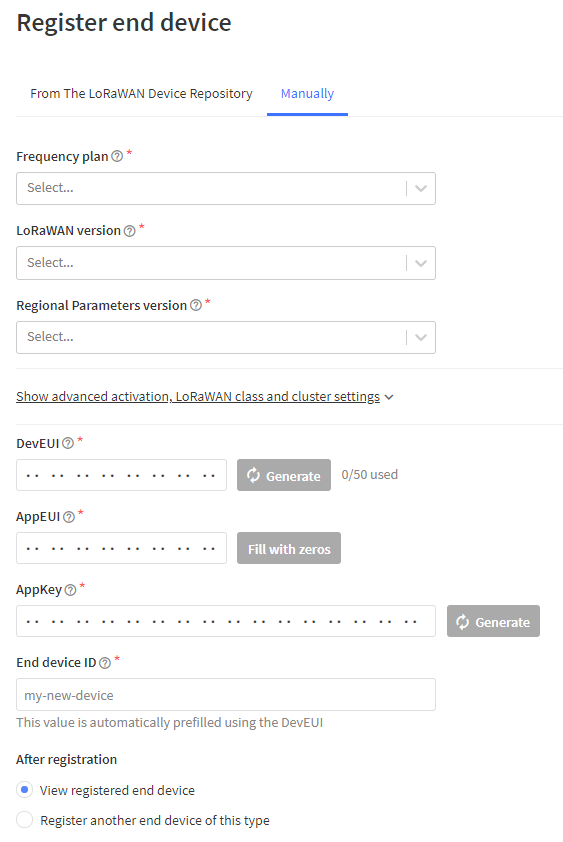
\includegraphics[width=.7\columnwidth]{Pictures/ttn-device.png} }
\lgf{\caption{Ajout d'un objet.}}
\lge{\caption{Adding an object.}}
\label{fig-ttn-device}
\end{figure}

\begin{itemize}
    \item 
        \lgf{Entrez le plan fréquence compatible avec votre région. En Europe, vous pouvez choisir d'avoir la voie descendante en SF9~\footnote{Le \acl{SF} definit la vitesse de transmission de l'information, elle diminue de moitié à chaque incrémentation doc le SF12 est 16 fois plus lent que le SF9, mais beaucoup plus robuste.} ou en SF12. Le premier est un bon compromis entre la portée et la durée d'émission ; le second est à choisir si votre objet est difficilement accessible (profondément enfoui ou loin d'une passerelle radio) ;}
        \lge{Enter the frequency plan compatible with your region. In Europe, you can choose to have the downlink in SF9~\footnote{The SF9~footnote defines the transmission speed of the information, it decreases by half at each increment doc the SF12 is 16 times slower than the SF9, but much more robust} or in SF12. The first one is a good compromise between the range and the transmission time; the second one is to be chosen if your object is difficult to reach (deeply buried or far from a radio gateway);}
    \item 
        \lgf{la version du protocole LoRaWAN compatible avec les LoPy  :\texttt{MAC V1.0.2}~;}
        \lge{the LoRaWAN protocol version compatible with LoPy :\texttt{MAC V1.0.2};}
    \item 
        \lgf{les paramètres de la couche physique du LoPy : \texttt{PHY V1.0.2 REV A}~;}
        \lge{the parameters of the physical layer of LoPy : \texttt{PHY V1.0.2 REV A};}
    \item 
        \lgf{Vous devez récupérer le \textit{devEUI} de votre LoPY en lançant sur Atom le programme \lprog{lorawan\_devEUI.py}{pycom} (cf. Listing~\vref{prog-devEUI})~;}
        \lge{You must recover the \textit{devEUI} of your LoPY by running on Atom the program \lprog{lorawan\_devEUI.py}{pycom} (cf. Listing~\vref{prog-devEUI});}
    \item 
        \lgf{mettez l'\textit{\Index{AppEUI}} à 0,}
        \lge{set the \textit{Index{AppEUI}} to 0,}
    \item 
        \lgf{et générez une clé de chiffrement \textit{\Index{AppKey}} et n'oubliez surtout pas de copier sa valeur quelque part, on en aura besoin pour configurer notre objet.}
        \lge{and generate an encryption key \textit{Index{AppKey}} and do not forget to copy its value somewhere, we will need it to configure our object.}
    
         \vspace{1em}

        \lgf{L'interface de TTN vous propose un identifiant pour l'objet basé sur son \textit{devEUI}. Vous pouvez le garder, à moins de vouloir quelque chose de plus explicite.}
        \lge{The TTN interface gives you an identifier for the object based on its \textit{devEUI}. You can keep it, unless you want something more explicit.}

         \vspace{1em}

        \lgf{Finally, click on \textit{register end device} to save your work.}

         \vspace{1em}

        \lgf{L'interface affiche une page récapitulative. Si vous avez oublié de le faire à l'étape précédente, copiez l'\textit{AppKey} pour la mettre dans le programme} 
        \lge{The interface displays a summary page. If you forgot to do it in the previous step, copy the \textit{AppKey} to put it in the program} \lprog{lorawan\_send\_and\_receive.py}{pycom}.
\end{itemize}

\lgf{\subsubsection*{Connexion de l'objet}}
\lge{\subsubsection*{Connecting the object}}

\pycomlst[firstline=1,lastline=10, firstnumber=1]{lorawan\_send\_and\_receive.py}

\lgf{Le programme \lprog{lorawan\_send\_and\_receive.py}{pycom} commence, comme \lprog{lorawan\_devEUI.py}{pycom}, par créer un objet \texttt{lora} et afficher le \textit{devEUI} de l'objet, c'est toujours partique pour le deboguage.}
\lge{The program \lprog{lorawan\_send\_and\_receive.py}{pycom} starts, like \lprog{lorawan\_devEUI.py}{pycom}, by creating a \texttt{lora} object and displaying the \textit{devEUI} of the object, it is always partique for debugging.}



\pycomnxt[firstline=12,lastline=18, firstnumber=12]{lorawan\_send\_and\_receive.py}

\lgf{On met dans deux variables, les identifiants présents sur le LNS de TTN, à savoir le \textit{app\_eui} que l'on avait mis à zéro et de \textit{app\_key} que l'on généré aléatoirement sur le site de TTN et que l'on vous avait demandé de copier quelque part.}
\lge{We put in two variables, the identifiers present on the LNS of TTN, namely the \textit{app\_eui} that we had put to zero and of \textit{app\_key} that we generated randomly on the site of TTN and that we had asked you to copy somewhere.}

\lgf{Pour éviter de manipuler des séquences binaires, ces valeurs sont vues comme des chaînes de caractères (des espaces peuvent être insérés pour plus de lisibilité, la fonction \texttt{replace} permet de les éliminer). La séquence binaire est obtenue grâce à la fonction \pfunction{binascii}{unhexlify}.}
\lge{To avoid manipulating binary sequences, these values are seen as strings (spaces can be inserted for more readability, the function \texttt{replace} allows to eliminate them). The binary sequence is obtained with the function \pfunction{binascii}{unhexlify}.}

\pycomnxt[firstline=19,lastline=20, firstnumber=19]{lorawan\_send\_and\_receive.py}

\lgf{On arrête le clignotement périodique bleu de la LED du LoPy en appelant la pfunction{pycom}{heartbeat} avec l'argument \texttt{False}. Puis on allume la LED en blanc avec la fonction \pfunction{pycom}{rgbled}. L'argument donne l'intensité des trois composantes Rouge, Vert et Bleu. }
\lge{We stop the periodic blue flashing of the LoPy LED by calling the pfunction{pycom}{heartbeat} with the argument \texttt{False}. Then the LED is lit in white with the function pfunction{pycom}{rgbled}. The argument gives the intensity of the three components Red, Green and Blue. }


\lgf{La LED va nous permettre de suivre pas à pas l'état du LoPy.}
\lge{The LED will allow us to follow the status of the LoPy step by step.}

\pycomnxt[firstline=22,lastline=30, firstnumber=22]{lorawan\_send\_and\_receive.py}

\lgf{Le LoPy effectue la connexion au réseau, cette procédure est appelée \textit{\Index{Join}}. Elle correspond à l'émission d'un message vers le LNS. Si celui-ci reconnaît et accepte l'objet, il renverra quelques secondes plus tard un message \texttt{Accept}. Cette phase permet à l'Objet d'obtenir les clés de chiffrement des messages et une adresse plus courte appelé \textit{\Index{devAddr}}.}
\lge{The LoPy makes the connection to the network, this procedure is called \textit{Index{Join}}. It corresponds to the emission of a message towards the LNS. If this one recognizes and accepts the object, it will return a few seconds later a message \texttt{Accept}. This phase allows the Object to obtain the encryption keys of the messages and a shorter address called \textit{Index{devAddr}}.}

\lgf{Pour se faire, le programme appelle la fonction \pfunction{lora}{join} avec les paramètres suivants~: }
\lge{To do this, the program calls the function \pfunction{lora}{join} with the following parameters~: }
\begin{itemize}
    \item 
        \lgf{le type de connexion, très souvent \ac{OTAA} pour récupérer dynamiquement les paramètres\footnote{Il existe aussi une méthode appelé \ac{ABP} qui consiste à configurer l'objet avec tous ses paramètres (comme pour Sigfox), mais elle est moins souple et moins adaptée à l'environnement LoRaWAN où plusieurs opérateurs coexistent sur les mêmes fréquences.},  }
        \lge{the type of connection, very often \ac{OTAA} to recover dynamically the parameters\footnote{There is also a method called \ac{ABP} which consists in configuring the object with all its parameters (like for Sigfox), but it is less flexible and less adapted to the LoRaWAN environment where several operators coexist on the same frequencies.},  }
        
    \item 
        \lgf{les paramètres nécessaires, à savoir l'\textit{AppEUI} et l'\textit{AppKey} que nous avons précédemment configurés.}
        \lge{the necessary parameters, namely the \textit{AppEUI} and the \textit{AppKey} that we have previously configured.}
        
    \item 
        \lgf{un temporisateur (\textit{timeout}). La valeur à 0 indique que l'objet va essayer de joindre le réseau jusqu'à ce que celui-ci l'accepte.}
        \lge{a timer (\textit{timeout}). The value of 0 indicates that the object will try to join the network until the network accepts it.}
\end{itemize}

         \vspace{1em}

\lgf{La fonction \pfunction{lora}{join} n'étant pas bloquante, la procédure de \textit{join} va se dérouler en tâche de fond. La fonction \pfunction{lora}{has\_joined} permet de suivre l'état du LoPy. D'où la boucle (lignes 26 à 28) dont on ne sortira que lorsque le LoPy sera accepter sur le réseau. }
\lge{As the function \pfunction{lora}{join} is not blocking, the procedure of \textit{join} will run in the background. The function \pfunction{lora}{has\_joined} allows to follow the state of the LoPy. Hence the loop (lines 26 to 28) from which we will only exit when the LoPy is accepted on the network. }


\lgf{Toutes de 2.5 seconde un message sera affiché pour dire qu'il est toujours en attente d'une réponse. Ces messages ne sont absolument pas synchronisés avec l'envoi des trames \texttt{Join} qui ont lieu toutes les 15 secondes.}
\lge{Every 2.5 seconds a message will be displayed to say that it is still waiting for a response. These messages are absolutely not synchronized with the sending of the frames \texttt{Join} which take place every 15 seconds.}

\lgf{L'extinction de la LED (ligne 30) indique que le LoPy a joint le réseau LoRaWAN.}
\lge{The extinction of the LED (line 30) indicates that the LoPy has joined the LoRaWAN network.}

\pycomnxt[firstline=32,lastline=34, firstnumber=32]{lorawan\_send\_and\_receive.py}

\lgf{Le programme ouvre la socket, le premier paramètre est \texttt{\Index{AF\_LORA}} pour indiquer que l'on utilise le protocole LoRaWAN. Les deux lignes suivantes, avec les fonctions \pfunction{socket}{setsockopt}, permettent de configurer des paramètres LoRaWAN, comme~:}
\lge{The program opens the socket, the first parameter is \texttt{Index{AF\_LORA}} to indicate that the LoRaWAN protocol is used. The next two lines, with the functions \pfunction{socket}{setsockopt}, allow to configure LoRaWAN parameters, like:}

\begin{itemize}
\item 
    \lgf{le \ac{DR}. Sous ce terme, plusieurs paramètres des la couche physique sont réunis. Plus le \ac{DR} est élevé, plus la transmission est rapide. En contre partie, elle est moins robuste et peut porter moins lion. Le \ac{DR} varie entre 0 et 6.}
    \lge{le \ac{DR}. Under this term, several parameters of the physical layer are gathered. The higher the \ac{DR}, the faster the transmission. In counterpart, it is less robust and can carry less lion. The \ac{DR} varies between 0 and 6.}
\item 
    \lgf{la capacité de LoRaWAN a acquitter les trames. Il n'est pas recommandé de l'activer car cela induit des émissions qui sont prises en compte dans le calcul du \Index{Duty Cycle} (voir chapitre~\vref{chap-star}).}
    \lge{the capacity of LoRaWAN to acknowledge frames. It is not recommended to activate it because it induces emissions which are taken into account in the calculation of the duty cycle (see chapter~\vref{chap-star}).}
\end{itemize}



\pycomnxt[firstline=36,lastline=46, firstnumber=36]{lorawan\_send\_and\_receive.py}

\lgf{On entre dans une boucle sans fin pour envoyer et recevoir périodiquement des messages~:}
\lge{We enter an endless loop to send and receive messages periodically:}

\begin{itemize}
    \item 
        \lgf{ligne 37, la LED éclaire en rouge pour indiquer une transmission.}
        \lge{ligne 37, la LED éclaire en rouge pour indiquer une transmission.}
        
    \item 
        \lgf{ligne 38, les appels aux sockets sont rendu bloquant, c'est-à-dire qu'il ne finiront que quand l'action sera effectuée par la couche inférieure.}
        \lge{line 38, the calls to the sockets are made blocking, i.e. they will finish only when the action is performed by the lower layer.}
    \item 
        \lgf{ligne 39, par contre au bout de 10 secondes d'attente une erreur sera déclanchée.}
        \lge{line 39, but after 10 seconds of waiting an error will be triggered.}
    \item 
        \lgf{ligne 41, on récupère cette erreur grâce aux instructions \texttt{\Index{try}} et \texttt{\Index{except}} de Python. Si l'appel à \pfunction{socket}{send} reste bloqué plus des 10 secondes, le traitement de l'exception affiche \texttt{timeout in sending}. Cet événement est rare et est causé par une défaillance locale à la couche 2\footnote{Il faut rester vigilant sur cette erreur, par exemple si l'on essaie d'envoyer un entier sans sérialisation, cela conduira à une erreur qui sera prise en compte de cette manière.}.}
        \lge{line 41, we recover this error thanks to the instructions \texttt{\Index{try}} and \texttt{\Index{except}} of Python. If the call to \pfunction{socket}{send} remains blocked for more than 10 seconds, the exception processing displays \texttt{timeout in sending}. This event is rare and is caused by a local failure at layer 2\footnote{You have to be careful with this error, for example if you try to send an integer without serialization, it will lead to an error which will be taken into account in this way.}.}
    \item 
        \lgf{ligne 46 dans tous les cas, la LED passe en bleu.}
        \lge{line 46 in all cases, the LED turns blue.}
\end{itemize}

\pycomnxt[firstline=49,lastline=59, firstnumber=49]{lorawan\_send\_and\_receive.py}

\lgf{Finalement, on attend des données. Dans le mode le plus fréquent de LoRaWAN, un équipement ne peut recevoir des données que dans une courte fenêtre après une émission. Si des données arrivent en dehors de cette fenêtre, le LNS mémorise l'information et la transmettra quand il recevra une trame de l'objet. Cela permet d'économiser beaucoup d'énergie car le capteur peut dormir de ses deux oreilles, il sait qu'il ne manquera pas une information.}
\lge{Finally, data is expected. In the most common mode of LoRaWAN, a device can only receive data within a short window after a transmission. If data arrives outside this window, the LNS stores the information and will transmit it when it receives a frame from the object. This saves a lot of energy because the sensor can sleep soundly, it knows that it will not miss any information.}


\lgf{La voie descendante est une ressource rare, et il ne faut généralement pas trop l'utiliser\footnote{TTN ne facture pas les données descendantes, mais d'autres opérateurs le font, faites attention si vous adaptez ces exemples à d'autres environnements, car dans les premiers tests, nous utiliseront la voie de retour.}, donc il ne devrait pas y avoir souvent de messages en retour. Sauf ici, pour tester toute la chaîne de transmission~:}
\lge{Downlink is a scarce resource, and should generally not be overused\footnote{TTN does not charge for downstream data, but other operators do, so be careful if you adapt these examples to other environments, because in the first tests we will use the return path.}, so there shouldn't be many return messages. Except here, to test the whole transmission chain:}

\begin{itemize}
    \item 
        \lgf{ligne 49, l'appel à \pfunction{socket}{recv} est aussi bloquant tant que des données ne sont pas arrivées. }
        \lge{line 49, the call to \pfunction{socket}{recv} is also blocking until data has arrived. }
    \item 
        \lgf{lignes 51 et 52, si des données arrivent, elles sont affichées et la LED passe au vert.}
        \lge{lines 51 and 52, if data arrives, it is displayed and the LED turns green.}
      
    \item 
        \lgf{lignes 53 à 55, si aucune données arrivent, le temporisateur se déclenche au bout de 10 secondes générant l''exception. Un message averti l'utilisateur de l'absence de données et la LED est éteinte.}
        \lge{lines 53 to 55, if no data arrive, the timer is triggered after 10 seconds generating the exception. A message warns the user of the absence of data and the LED is turned off.}
\end{itemize}

         \vspace{1em}

\lgf{Si tout va bien, qu'une passerelle radio est à portée de votre objet, le programme  \lprog{lorawan\_send\_and\_receive.py}{pycom} va se connecter au réseau après avoir affiché 3 fois \texttt{Not yet joined...}~:}
\lge{If all is well, and a radio gateway is in range of your object, the program \lprog{lorawan\_send\_and\_receive.py}{pycom} will connect to the network after displaying \texttt{Not yet joined...}~ 3 times:}


\begin{termc}[backgroundcolor=\color{gray!10}, basicstyle=\ttfamily\small, escapechar=@] 
>>> Running lorawan_send_and_receive.py

>>>
>>>
devEUI:  b'70b3d54994c61237'
Not yet joined...
Not yet joined...
Not yet joined...
timeout in receive
timeout in receive
\end{termc}


\noindent 
\lgf{correspondant au 5 secondes prévues par le standard avant d'envoyer le message d'acceptation de l'objet. }
\lge{corresponding to the 5 seconds provided by the standard before sending the message of acceptance of the object. }


\lgf{La LED passe du blanc au rouge indiquant qu'un message a été émis puis doit s'éteindre et le message \texttt{timeout in receive} est affiché indiquant que l'Objet n'a pas reçu de message en réponse à son émission.}
\lge{The LED changes from white to red indicating that a message has been sent and then should go out and the message \texttt{timeout in receive} is displayed indicating that the Object has not received a message in response to its transmission.}


\lgf{\subsubsection{Analyse des traces}}
\lge{\subsubsection{Trace analysis}}


\lgf{Côté LNS, il est possible de voir le trafic sur la page résumant les caractéristiques de l'objet dans la fenêtre \textit{live data} (cf. figure~\vref{fig-lora-join}).}
\lge{On the LNS side, it is possible to see the traffic on the page summarizing the characteristics of the object in the \textit{live data} window (see figure~\vref{fig-lora-join}).}


\begin{figure}[tbp]
\centerline{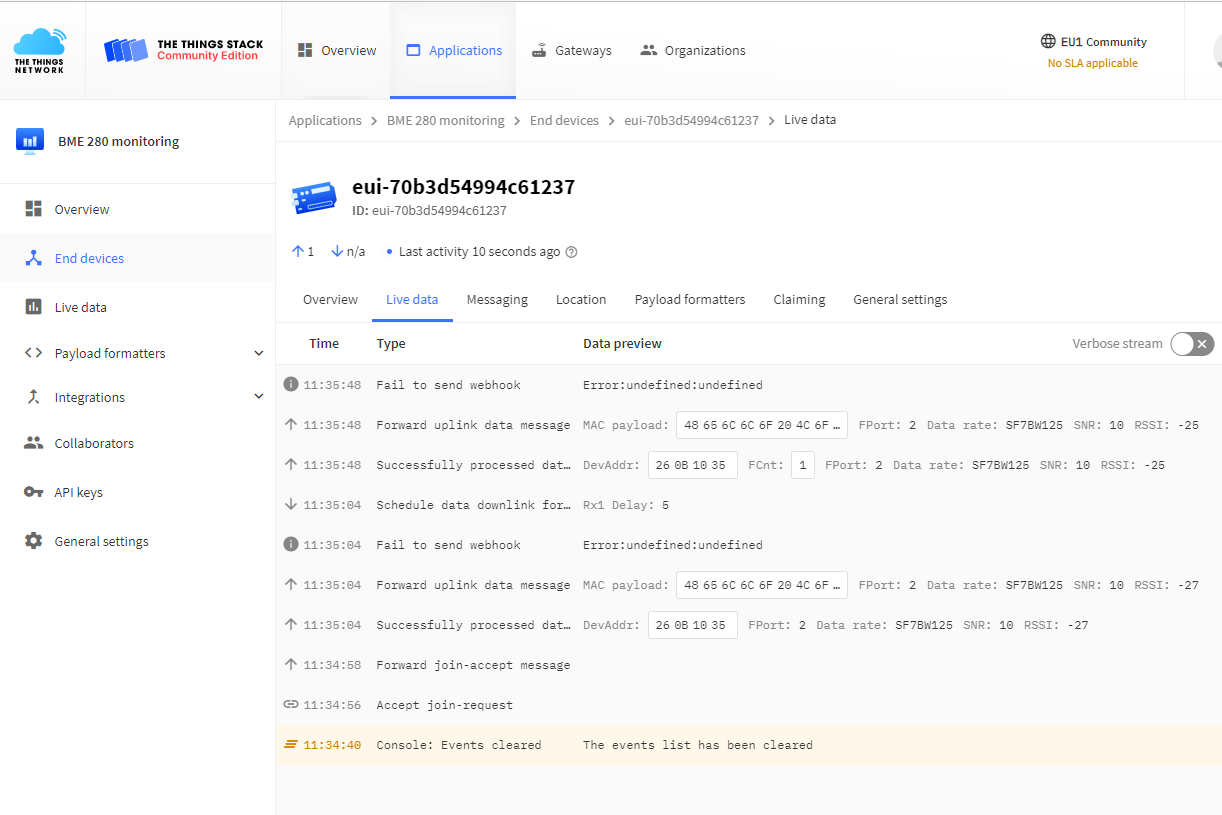
\includegraphics[width=.7\columnwidth]{Pictures/lora-join.png} }
\lgf{\caption{Trace d'un objet.}}
\lge{\caption{Trace of an object.}}
\label{fig-lora-join}
\end{figure}

\lgf{Les événements sur la figure se lisent de bas en haut comme le confirme l'horodatage, en cliquant sur la ligne correspondante, TTN affiche les messages JSON utilisés par le LNS pour traiter l'information. On y retrouve les données échangées~:}
\lge{The events on the figure are read from bottom to top as confirmed by the timestamp, by clicking on the corresponding line, TTN displays the JSON messages used by the LNS to process the information. The data exchanged is shown:}


\begin{itemize}
    \item 
        \lgf{L'événement \textit{Accept \Index{Join-request}} indique que le LNS a reçu le message Join de l'objet, indiquant qu'il voulait rejoindre le réseau. Le LNS l'a traité, a vérifié qu'il y avait un objet déclaré avec le bon \textit{\Index{devEUI}} et que l'\textit{\Index{AppKey}} utilisée par l'objet pour signer sa demande était identique à la valeur configurée. Dans la trace suivante, on peut retrouver le \textit{\Index{devEUI}} de l'objet et la \textit{\Index{devAddr}}, qui lui a été attribuée temporairement. Cette dernière sera utilisée par la suite.}
        \lge{The event \textit{Accept \Index{Join-request}} indicates that the LNS received the Join message from the object, indicating that it wanted to join the network. The LNS treated it, verified that there was an object declared with the good \textit{Index{devEUI}} and that the \textit{Index{AppKey}} used by the object to sign its request was identical to the configured value. In the following trace, we can find the \textit{\Index{devEUI}} of the object and the \textit{\Index{devAddr}}, which was temporarily assigned to it. The latter will be used later.}
    
\begin{termc}[backgroundcolor=\color{blue!10}, basicstyle=\ttfamily\small, escapechar=@] 
    "device_ids": {
        "device_id": "eui-70b3d54994c61237",
        "application_ids": {
          "application_id": "plido-appl"
        },
        "dev_eui": "70B3D54994C61237",
        "join_eui": "0000000000000000",
        "dev_addr": "260B1035"
      }
\end{termc}

    \item 
        \lgf{L'événement \textit{Forward \Index{Join-accept} message} indique que le LNS envoie un message d'acceptation à l'Objet. Ce message est différé de 5 secondes pendant lesquelles l'Objet dort. }
        \lge{The event \textit{Forward \Index{Join-accept} message} indicates that the LNS sends an acceptance message to the Object. This message is delayed by 5 seconds during which the Object sleeps. }
    
    \item  
        \lgf{L'événement \textit{Successfully processed data message} montre que le LNS a reçu correctement le message de données émis par l'Objet. La trace donne des indications sur certains paramètres physique, tels que le \acl{SF} (ici SF7 soit la modulation la plus rapide et la moins robuste), le SNR qui indique le ratio entre la puissance du signal reçu par rapport au bruit et le \ac{RSSI} donnant la force du signal.   }
        \lge{The event \textit{Successfully processed data message} shows that the LNS received correctly the data message emitted by the Object. The trace gives indications on certain physical parameters, such as the SF (here SF7 is the fastest and least robust modulation), the SNR which indicates the ratio between the power of the received signal compared to the noise and the RSSI giving the strength of the signal. }
    
    \item  
        \lgf{L'événement \textit{Forward uplink data message} donne plus d'information sur le message et son contenu. Le champs \texttt{frm\_payload} donne le contenu déchiffré par le LNS mais codé en \Index{base64}. On y retrouve le message d'origine \texttt{Hello LoRa}. }
        \lge{The event \textit{Forward uplink data message} gives more information about the message and its content. The field \texttt{frm\_payload} gives the contents decrypted by the LNS but encoded in \Index{base64}. One finds there the original message \texttt{Hello LoRa}. }
        
\begin{termc}[backgroundcolor=\color{blue!10}, basicstyle=\ttfamily\small, escapechar=@] 
    "uplink_message": {
      "session_key_id": "AX4VNOuMbClcPKF63sKy6A==",
      "f_port": 2,
      "frm_payload": "SGVsbG8gTG9SYQ==",
      "rx_metadata": [
        {
          "gateway_ids": {
            "gateway_id": "gateway-lo",
            "eui": "B827EBFFFE08F8A8"
          },
          "time": "2022-01-01T10:35:04.247807Z",
          "timestamp": 2661650827,
          "rssi": -27,
          "channel_rssi": -27,
          "snr": 10,
          "uplink_token": "ChgKFgoKZ2F0ZX....",
          "channel_index": 1
        }
      }
\end{termc}


\end{itemize}


    
\Question{\lgf{Mauvais appKey}\lge{Bad appKey}}
{
\lgf{Quel message de trace obtenez vous du LNS, si l'Objet n'est pas configuré avec le même \yexyit{\Index{AppKey}} que le LNS~?}
\lge{What trace message do you get from the LNS, if the Object is not configured with the same \yexyit{Index{AppKey}} as the LNS~?}

}
{
\texttt{12:52:11 Join-request to cluster-local Join Server failed MIC mismatch}\\
\texttt{12:52:01 Join-request to cluster-local Join Server failed MIC mismatch}\\
\texttt{12:51:51 Join-request to cluster-local Join Server failed MIC mismatch}\\

}

\Question{\lgf{Autonomie}\lge{Autonomy}}
{
\lgf{Quel impact sur les batteries~?}
\lge{What impact on batteries?}
}
{
\lgf{Le LoPy va émettre périodiquement tous les 10 secondes un message de type \Index{Join-request}. Le but est pouvoir se connecter, même si la transmission n'est pas optimale. mais en cas de mauvaise configuration, cela va se traduire par une occupation plus importante du réseau, mais surtout un impact sur l'autonomie de l'Objet.}
\lge{The LoPy will emit periodically every 10 seconds a message of type \Index{Join-request}. The goal is to be able to connect, even if the transmission is not optimal. But in case of bad configuration, it will result in a higher occupation of the network, but especially an impact on the autonomy of the Object.}
}
\lgf{Le \Index{fPort} que l'on retrouve dans les trames de données LoraWAN permet d'indiquer le programme qui va traiter l'information. La valeur 0 est spéciale et indique une trame de configuration de la couche LoRaWAN, les autres valeurs jusquà 223 désignent des applications spécifiques. Bien qu'il soit peu utilisé, il est parfois utile de la changer. }
\lge{The index{fPort} found in the LoraWAN data frames indicates the program that will process the information. The value 0 is special and indicates a configuration frame of the LoRaWAN layer, the other values up to 223 indicate specific applications. Although it is little used, it is sometimes useful to change it. }


\Question{fPort}
{
\lgf{Dans les traces précédentes, quelle est la valeur du fPort par défaut utilisé par le LoPy~? }
\lge{In the previous traces, what is the value of the default fPort used by the LoPy? }
}
{\texttt{  "f\_port": 2,}}

\Question{\lgf{Changement de fPort}\lge{Changing the fPort}}
{
\lgf{L'instruction \pfunction{socket}{bind} permet de modifier le \Index{fPort} pour une transmission. Modifiez le programme pour utiliser le fPort 10 et vérifiez l'effet dans les traces de TTN. }
\lge{The instruction \pfunction{socket}{bind} allows to modify the \Index{fPort} for a transmission. Modify the program to use fPort 10 and check the effect in the TTN traces. }
}
{
\lgf{Le programme doit être modifié par exemple après les instructions \pfunction{socket}{setsockopt} en ajoutant la ligne~:\\
\texttt{s.bind(10)}\\
}
\lge{The program must be modified, for example, after the instructions \pfunction{socket}{setsockopt} by adding the line:\\
\texttt{s.bind(10)}\\
}
}

\lgf{\subsubsection{Configuration du connecteur}}
\lge{\subsubsection{Connector configuration}}

\lgf{Le LNS n'a pas été configuré pour envoyer le message à un Serveur d'Application (\acl{AS}). Comme pour \Index{Sigfox}, il faut définir une URI pour indiquer au LNS où poster les données.}
\lge{The LNS has not been configured to send the message to an Application Server (\acl{AS}). As for \Index{Sigfox}, a URI must be defined to tell the LNS where to post the data.}

         \vspace{1em}


\lgf{Pour configurer un connecteur, il faut aller sur le menu de gauche \textit{Integrations}. TTN propose des intégrations directes avec des services cloud existants, mais il est également possible de configurer son propre connecteur~:}
\lge{To configure a connector, go to the left menu \textit{Integrations}. TTN offers direct integrations with existing cloud services, but it is also possible to configure your own connector:}


\begin{itemize}
    \item 
        \lgf{via \Index{MQTT}, TTN joue le rôle de \Index{\textit{broker}} et fourni le nom du \Index{topic} et le secret.}
        \lge{through \Index{MQTT}, TTN plays the role of \Index{textit{broker}} and provides the name of the \Index{topic} and the secret.}
        
    \item 
        \lgf{en stockant localement des données par le choix \textit{\Index{Storage integration}} et en y accédant par une requête GET, comme Sigfox le propose (cf. chapitre~\vref{chap-sigfox-GET}). Cela permet de recevoir les données si l'on est situé derrière un \ac{NAT}, mais rend la réception asynchrone puisque l'application doit interroger régulièrement le serveur de TTN.}
        \lge{by storing data locally by the choice \textit{Index{Storage integration}} and by accessing it by a GET request, as Sigfox proposes (cf. chapter~\vref{chap-sigfox-GET}). That makes it possible to receive the data if one is located behind a NAT, but makes the reception asynchronous since the application must regularly question the TTN server.}
        
    \item 
        \lgf{en configuration une URI sur le serveur pour que celui-ci produit une requête POST quand une trame de donnée est reçue (choix \textit{\Index{Webhooks}}).}
        \lge{by configuring a URI on the server so that it produces a POST request when a data frame is received (choice \textit{\Index{Webhooks}}).}
\end{itemize}

         \vspace{1em}

\lgf{Nous allons également privilégier pour TTN ce dernier mode de fonctionnement, car si il nécessite une configuration du \ac{NAT}, il permet de recevoir les données de manière synchrone lorsqu'elles sont traitées par le LNS.}
\lge{We will also favour this last mode of operation for TTN, because if it requires a configuration of the LNS, it makes it possible to receive the data in a synchronous way when they are processed by the LNS.}



\lgf{Il faut cliquer sur \Index{Webhooks}. Un certain nombre de services sont proposés, mais nous allons définir le nôtre à l'instar de ce que nous avons fait avec Sigfox (cf. chapitre~\vref{chap-sigfox-POST}). Pour préparer la connectivité, il est nécessaire~:}
\lge{You have to click on \Index{Webhooks}. A certain number of services are proposed, but we will define our own following the example of what we did with Sigfox (cf. chapter~\vref{chap-sigfox-POST}). To prepare the connectivity, it is necessary:}

\begin{itemize}
    \item 
        \lgf{Si vous êtes dans le cloud, l'adresse s'obtient en tapant la commande \texttt{\Index{ifconfig}}.}
        \lge{If you are in the cloud, the address is obtained by typing the command \texttt{\Index{ifconfig}}.}
        
    \item 
        \lgf{Si vous êtes derrière une box ou le routeur de votre fournisseur d'accès, vous avez une adresse privée. Un site web comme \url{myip.wtf} vous retournera l'adresse IPv4 publique. Vous devez ensuite configurer votre router d'accès pour qu'il envoie les paquets TCP ayant le numéro de port 9999 à votre ordinateur.}
        \lge{If you are behind a box or your ISP's router, you have a private address. A web site like \url{myip.wtf} will return the public IPv4 address. You must then configure your access router to send TCP packets with port number 9999 to your computer.}
\end{itemize}

         \vspace{1em}


\lgf{Cela va permette de former l'URI suivante~:}
\lge{This will form the next URI:}

\begin{termc}[backgroundcolor=\color{blue!10}, basicstyle=\ttfamily\small, escapechar=@]
http://@\textit{aaa.bbb.ccc.ddd}@:9999/ttn
\end{termc}

\noindent 
\lgf{où \textit{aaa.bbb.ccc.ddd} représente l'adresse IP publique de votre équipement. Comme cette adresse peut changer au cours du temps, il est préférable d'utiliser un service de DNS dynamique pour obtenir un nom de domaine plus stable sur la durée.}
\lge{where \textit{aaa.bbb.ccc.ddd} represents the public IP address of your equipment. As this address can change over time, it is preferable to use a dynamic DNS service to obtain a more stable domain name over time.}


         \vspace{1em}

\lgf{La page listant les \textit{\Index{Webhooks}} associés à l'application est vide. Il faut cliquer sur \textit{} pour en ajouter un nouveau, il convient de choisir \textit{Custom webhook}, les autres définissent les connecteurs vers des services de gestion des données (cf. figure~\vref{fig-ttn-webhook}).}
\lge{The page listing the \textit{Index{Webhooks}} associated with the application is empty. You must click on \textit{} to add a new one, it is advisable to choose \textit{Custom webhook}, the others define the connectors to data management services (cf. figure~\vref{fig-ttn-webhook}).}


\begin{figure}[tbp]
\centerline{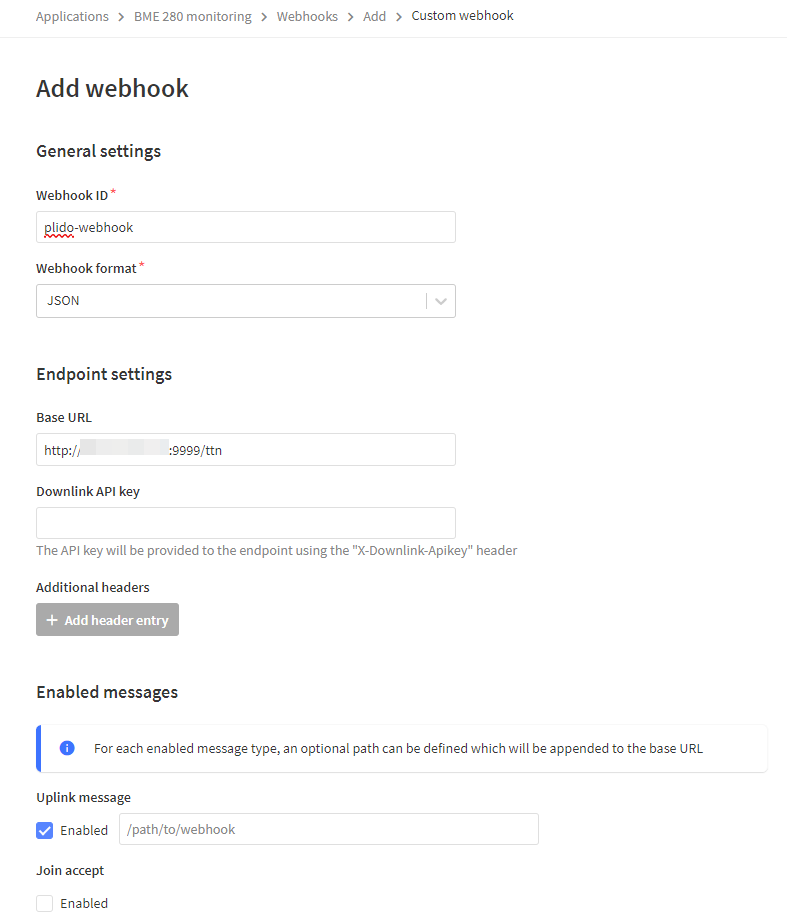
\includegraphics[width=.7\columnwidth]{Pictures/ttn-webhook.png} }
\lgf{\caption{Configuration d'un webhook.}}
\lge{\caption{Webhook configuration.}}
\label{fig-ttn-webhook}
\end{figure}

\lgf{Dans ce menu, il faut indiquer~:}
\lge{In this menu, you should indicate:}

\begin{itemize}
    \item 
        \lgf{l'identifiant du webhook~:}
        \lge{the webhook identifier:}
    \item 
        \lgf{le format JSON~:}
        \lge{the JSON format:}
    \item 
        \lgf{l'URI que nous venons de construire~:}
        \lge{the URI that we have just built:}
    \item 
        \lgf{il n'est pas nécessaire pour l'instant de remplir la \textit{Download API Key} qui servira pour envoyer des données à l'Objet. Nous y reviendrons par la suite.}
        \lge{it is not necessary for the moment to fill the \textit{Download API Key} which will be used to send data to the Object. We will come back to this later.}
    \item 
        \lgf{il faut choisir les événements qui déclencheront une requête POST. Dans notre cas, on ne choisi que la récéption d'un message montant (\textit{Uplink message}).  On peut compléter le chemin de l'URI précédemment définie avec des éléments qui permettrons au serveur REST de mieux identifier le type de requête. Dans notre cas, cela n'est pas nécessaire. \texttt{/ttn} identifie par conséquent les messages reçus par le LNS des Objets.}
        \lge{you have to choose the events that will trigger a POST request. In our case, we will only choose the reception of an upload message (\textit{Uplink message}).  We can complete the path of the previously defined URI with elements that will allow the REST server to better identify the type of request. In our case, this is not necessary. \texttt{/ttn} therefore identifies the messages received by the Objects LNS.}
\end{itemize}

\lgf{Une fois le \textit{webhook} validé, le programme \pprog{generic\_relay.py}{plido-tp3} doit être lancé. Il va créer un serveur Web qui va attendre les requêtes POST du LNS de TTN.}
\lge{Once the \textit{webhook} validated, the program \pprog{generic\_relay.py}{plido-tp3} must be launched. It will create a Web server which will wait for the POST requests of the LNS of TTN.}


         \vspace{1em}

 \pythonnxt[firstline=93,lastline=128, firstnumber=93   ]{generic\_relay.py}
 
\lgf{Ce programme utilise le module \Index{Flask} pour créer un serveur Web. Il associe le chemin \texttt{/ttn} à la fonction \texttt{get\_from\_ttn} pour les requêtes de type POST (lignes 93 et 94). Quand une requête de ce type arrive, la variable 
\texttt{fromGW} contient l'objet JSON\footnote{convertie implicitement en dictionnaire Python.} (ligne 95). Si elle contient la clé \texttt{uplink\_message}, les données sont extraites (ligne 100) pour être envoyé au travers de l'interface \textit{\Index{loopback}}  grâce à la fonction \texttt{\Index{forward\_data}} à un programme qui les traite. Si cette fonction retourne la valeur \texttt{None}, le programme ne souhaite pas répondre à l'Objet, le serveur Web acquitte positivement (code \texttt{200}) la requête venant du LNS (ligne 130 et 131).}
\lge{This program uses the module \Index{Flask} to create a Web server. It associates the path \texttt{/ttn} with the function \texttt{get\_from\_ttn} for requests of type POST (lines 93 and 94). When a request of this type arrives, the variable 
\texttt{fromGW} variable contains the JSON object\footnote{converted implicitly into a Python dictionary.} (line 95). If it contains the key \texttt{uplink\_message}, the data are extracted (line 100) to be sent through the interface \textit{\Index{loopback}} thanks to the function \texttt{\Index{forward\_data}} to a program which processes them. If this function returns the value \texttt{None}, the program does not wish to answer the Object, the Web server acknowledges positively (code \texttt{200}) the request coming from the LNS (line 130 and 131).}

\label{chap—forward-data}
 \pythonnxt[firstline=27,lastline=50, firstnumber=27]{generic\_relay.py}


\lgf{Si le mode \texttt{verbose} est activé, le message à envoyer au programme de traitement des données est affiché en hexadécimal grâce à la fonction \pfunction{binascii}{hexlify} (lignes 33 et 34). Puis le message est effectivement émis (ligne 35)\footnote{l'adresse du destinataire et le port sont configurés lors de l'analyse des paramètres.}}
\lge{If the \texttt{verbose} mode is activated, the message to be sent to the data processing program is displayed in hexadecimal thanks to the function \pfunction{binascii}{hexlify} (lines 33 and 34). Then the message is actually sent (line 35)\footnote{the address of the recipient and the port are configured during the analysis of the parameters.}}


\lgf{Pour attendre une réponse qui n'est pas systématique, on ne peut pas utiliser l'appel \pfunction{socket}{recvfrom} car celui-ci est bloquant. A la place, on utilise l'appel \pfunction{select}{select} du module du même nom. Il permet d'attendre sur plusieurs événements à la fois provenant de différentes sockets (ligne 37) où~:}
\lge{To wait for a response that is not systematic, we cannot use the \pfunction{socket}{recvfrom} call because it is blocking. Instead, we use the \pfunction{select}{select} call of the module of the same name. It allows to wait on several events at the same time coming from different sockets (line 37) where~:}

\begin{itemize}
    \item  
        \lgf{\texttt{inputs} est un tableau des sockets pouvant avoir reçu des données. Dans notre cas (ligne 30) il est initialisé avec la socket dialoguant avec le programme traitant les données~;}
        \lge{\texttt{inputs} is an array of sockets that may have received data. In our case (line 30) it is initialized with the socket talking to the program processing the data~;}
        
    \item  
        \lgf{\texttt{outputs} est un tableau qui contient les sockets dans lesquelles il serait possible d'écrire. Dans notre cas, ce tableau est vide (ligne 31).}
        \lge{\texttt{outputs} is an array which contains the sockets in which it would be possible to write. In our case, this array is empty (line 31).}
        
    \item  
        \lgf{le troisième concerne les exceptions. Dans notre cas, on répète le tableau des sockets \texttt{inputs}}
        \lge{the third one concerns the exceptions. In our case, we repeat the table of sockets \texttt{inputs}}
        
    \item  
        \lgf{finalement le quatrième praramètre indique la durée d'attente dans la fonction \pfunction{select}{select}. Dans notre cas, il est fixé à 0.1 seconde. ce temps est a la fois compatible avec une réponse du programme de traitement des données, et la réponse que l'on doit envoyer au LNS pour que la réponse soit associée au message montant.}
        \lge{finally the fourth parameter indicates the waiting time in the function \pfunction{select}{select}. In our case, it is set to 0.1 second. This time is both compatible with a response from the data processing program, and the response that must be sent to the LNS so that the response is associated with the upstream message.}
\end{itemize}

\lgf{\pfunction{select}{select} retourne dans un tuple de trois éléments, la ou les sockets qui ont déclenché son retour. Dans notre cas, se sont~:}
\lge{\pfunction{select}{select} returns in a tuple of three elements, the socket(s) that triggered its return. In our case, these are:}


\begin{itemize}
    \item 
        \lgf{soit l'expiration du temporisateur, dans ce cas, la variable \texttt{readable} qui contient la liste des sockets ayant recues des données est vide (ligne 39) et la valeur \texttt{None} est retournée.}
        \lge{either the expiration of the timer, in this case, the variable \texttt{readable} which contains the list of sockets having received data is empty (line 39) and the value \texttt{None} is returned.}
        
    \item 
        \lgf{soit des données qui sont arrivées dans une ou plusieurs socket. la variable \texttt{readable} contient le tableau de ces sockets. La variable \texttt{s} contient la première socket du tableau, les données sont lues et envoyées en retour.}
        \lge{or data which arrived in one or more sockets. The variable \texttt{readable} contains the array of these sockets. The variable \texttt{s} contains the first socket of the array, the data are read and sent back.}
\end{itemize}


         \vspace{1em}

\lgf{Le programme \pprog{generic\_relay.py}{plido-tp3}, lancé avec l'option \texttt{-v} montre de manière synthétique le trafic. }
\lge{The program \pprog{generic\_relay.py}{plido-tp3}, launched with the option \texttt{-v} shows in a synthetic way the traffic. }



\begin{termc}[backgroundcolor=\color{palerod}, basicstyle=\ttfamily\small, escapechar=@]
>python3 generic_relay.py -v
--UP-> b'48656c6c6f204c6f5261'
no DW
63.34.43.96 - - [01/Jan/2022 18:27:45] "POST /ttn HTTP/1.1" 200 -
--UP-> b'48656c6c6f204c6f5261'
no DW
34.255.49.188 - - [01/Jan/2022 18:28:31] "POST /ttn HTTP/1.1" 200 -
\end{termc}

\lgf{Le contenu du message montant est affiché en hexadécimal et correspond au fameux contenu \texttt{Hello LoRa}. Comme il n'y a pas de réponse, \texttt{no DW} est ensuite affiché.}
\lge{The content of the rising message is displayed in hexadecimal and corresponds to the famous content \texttt{Hello LoRa}. As there is no answer, \texttt{no DW} is then displayed.}


\lgf{\subsubsection{Traitement des données}}
\lge{\subsubsection{Data processing}}

\lgf{La fonction \texttt{\Index{forward\_data}} du programme \pprog{generic\_relay.py}{plido-tp3} envoie les données à l'adresse de \textit{\Index{loopback}} \texttt{127.0.0.1} et sur le port \texttt{33033}\footnote{Ces deux valeurs peuvent être respectivement changées  en utilisant les arguments \texttt{-{}-forward\_address} et  \texttt{-{}-forward\_port}.}.}
\lge{The function \texttt{\Index{forward\_data}} of the program \pprog{generic\_relay.py}{plido-tp3} sends the data to the address of \texttt{127.0.0.1}\footnote{These two values can be respectively changed by using the arguments \texttt{-{}-forward\_address} and \texttt{-{}-forward\_por}.}.}



\lgf{Le programmme \pprog{display\_receive\_and\_send.py}{plido-tp3} traite les données de l'Objet.}
\lge{The program \pprog{display\_receive\_and\_send.py}{plido-tp3} processes the data of the Object.}


\pythonlst{display\_receive\_and\_send.py}

\lgf{Il attend les données sur le port 33033. La fonction \pfunction{socket}{recvfom} retourne les données stockées dans la variable \texttt{data} et l'adresse de celui qui a envoyé les données stockée dans la variable \texttt{addr}. Les données sont affichée ligne 9 et le message \texttt{Pleased to meet you} est retourné à l'émetteur, en ligne 10 grâce à la fonction \pfunction{socket}{sendto}.}
\lge{It waits for the data on port 33033. The function \pfunction{socket}{recvfom} returns the data stored in the variable \texttt{data} and the address of the one who sent the data stored in the variable \texttt{addr}. The data is displayed on line 9 and the message \texttt{Pleased to meet you} is returned to the sender, on line 10 thanks to the function \pfunction{socket}{sendto}.}

         \vspace{1em}

\lgf{En lançant le programme dans une nouvelle fenêtre, on reçoit correctement le message du LoPy.}
\lge{By launching the program in a new window, the LoPy message is correctly received.}

\begin{termc}[backgroundcolor=\color{palerod}, basicstyle=\ttfamily\small, escapechar=@]
>python3 display_receive_and_send.py
b'Hello LoRa'
\end{termc}

\lgf{En revanche, le programme \pprog{generic\_relay.py}{plido-tp3} produit une erreur.}
\lge{On the other hand, the program \pprog{generic\_relay.py}{plido-tp3} produces an error.}


\begin{termc}[backgroundcolor=\color{palerod}, basicstyle=\ttfamily\small, escapechar=@]
--UP-> b'48656c6c6f204c6f5261'
<-DW-- b'506c656173656420746f206d65657420796f7521'
63.34.43.96 - - [01/Jan/2022 19:06:51] "POST /ttn HTTP/1.1" @\textcolor{red}{500}@ -
Traceback (most recent call last):
...
\end{termc}

\lgf{Le message en retour a été reçu par la fonction \texttt{\Index{forward\_data}}, mais la voie descendante n'a pas encore été configurée. L'erreur est liée à l'absence du fichier \pprog{ttn\_config.py}{plido-tp3}, ligne 104, ce qui force Flask a retourner le status \texttt{500} et afficher les fonctions qui ont conduit à l'erreur.}
\lge{The return message was received by the function \texttt{\Index{forward\_data}}, but the downstream path has not yet been configured. The error is linked to the absence of the file \pprog{ttn\_config.py}{plido-tp3}, line 104, which forces Flask to return the status \texttt{500} and to display the functions which led to the error.}


\lgf{\subsubsection{Voie retour}}
\lge{\subsubsection{Return path}}

\lgf{Il n'y a aucun problème de sécurité quand le LNS envoie au serveur d'application des données reçues de capteurs, car l'endroit où il les transmet a été configuré par leur propriétaire. Par contre, dans l'autre sens, le LNS doit s'assurer que les données à transmettre à l'Objet, proviennent bien d'un serveur d'application autorisé.}
\lge{There is no security problem when the LNS sends data received from sensors to the application server, because the place where it transmits them has been configured by their owner. However, in the other direction, the LNS must ensure that the data to be transmitted to the Object comes from an authorized application server.}

\lgf{Comme pour Beebotte, une clé secrète va être utilisée. A cette clé, le LNS peut associer des droits pour plus ou mois limiter les accès. Dans le menu de gauche, cliquez sur \textit{API key} puis sur \textit{+ Add API Key}. Dans l'écran suivant, donnez un nom à votre clé et choisissez \textit{Grant Individual Right} pour limiter l'usage de la clé. Sélectionnez \textit{Write downlink application traffic} et validez. }
\lge{As for Beebotte, a secret key will be used. To this key, the LNS can associate rights to more or less limit access. In the left menu, click on \textit{API key} then on \textit{+ Add API Key}. In the next screen, give your key a name and choose \textit{Grant Individual Right} to limit the use of the key. Select \textit{Write downlink application traffic} and validate. }



         \vspace{1em}

\lgf{Recopiez la clé et confirmer que vous l'avez bien fait en validant \textit{I have copied the key}. Editez le fichier \pprog{ttn\_config.py}{plido-tp3} en y insérant la clé obtenue.}
\lge{Copy the key and confirm that you have done so by validating \textit{I have copied the key}. Edit the file \pprog{ttn\_config.py}{plido-tp3} by inserting the key obtained.}


\pythonlst{ttn\_config.py}

\begin{figure}[tbp]
\centerline{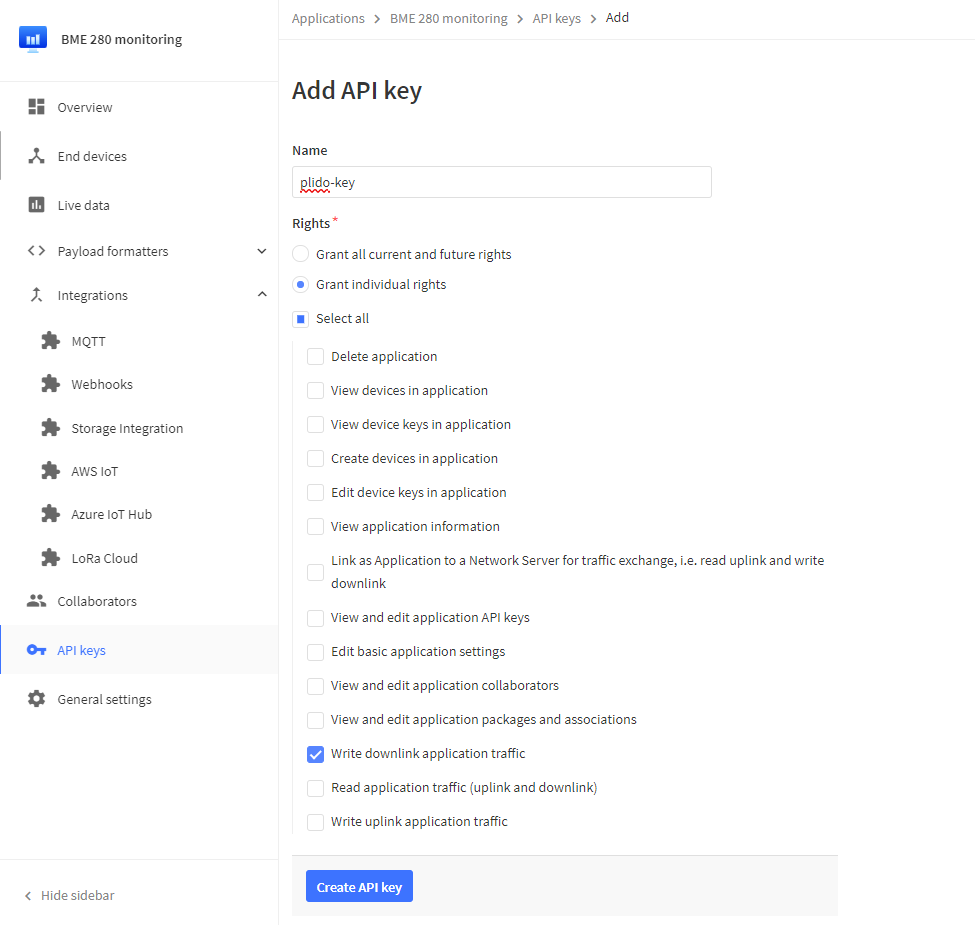
\includegraphics[width=.7\columnwidth]{Pictures/ttn-key.png} }
\lgf{\caption{Création d'une clé}}
\lge{\caption{Creating a key}}
\label{fig-ttn-key}
\end{figure}

\lgf{Relancez le programmme \pprog{generic\_relay.py}{plido-tp3}, le LoPy  affiche la réponse.}
\lge{Relaunch the program \pprog{generic\_relay.py}{plido-tp3}, the LoPy displays the answer.}


         \vspace{1em}

\lgf{Le listing suivant reprend la construction de la requête POST vers le LNS pour transporter le message descendant~:}
\lge{The following listing shows the construction of the POST request to the LNS to transport the descending message:}

 \pythonnxt[firstline=103,lastline=125, firstnumber=103]{generic\_relay.py}

\begin{itemize}
\item 
    \lgf{ligne 104, la clé autorisant l'envoi de message descendant est copié dans la variable \texttt{TTN\_Downlink\_Key}.}
    \lge{line 104, the key authorizing the sending of downlinked messages is copied into the variable \texttt{TTN\_Downlink\_Key}.}
    
\item 
    \lgf{lignes 106 à 110, le format JSON attendu par le LNS pour envoyer un message descendant est construit, plusieurs messages peuvent être envoyés à la fois, d'où l'utilisation d'un tableau. Chacun des éléments contient un \texttt{\Index{fPort}} qui est recopié du message montant et des données qui proviennent de la socket (variable \texttt{downlink} codé en base64.}
    \lge{lines 106 to 110, the JSON format expected by the LNS to send a downlink message is built, several messages can be sent at the same time, hence the use of an array. Each of the elements contains a \texttt{\Index{fPort}} which is copied from the upstream message and the data coming from the socket (variable \texttt{downlink} encoded in base64.}

\begin{termc}[backgroundcolor=\color{palerod}, basicstyle=\ttfamily\tiny, escapechar=@]
{'downlinks': [{'frm_payload': 'UGxlYXNlZCB0byBtZWV0IHlvdSE=', 'f_port': 10}]}
\end{termc}
\item 
    \lgf{lignes 111 à 116, l'URI pour accéder au service est construite. Elle contient deux éléments variables qui identifient l'application et l'Objet. Ceux-ci sont également extrait du message montant.}
    \lge{lines 111 to 116, the URI to access the service is constructed. It contains two variable elements which identify the application and the Object. These are also extracted from the upstream message.}
    
\begin{termc}[backgroundcolor=\color{palerod}, basicstyle=\ttfamily\tiny, escapechar=@]
https://eu1.cloud.thethings.network/api/v3/as/applications/plido-appl/devices/eui-70b3d54994c61237/down/push
\end{termc}
\item 
    \lgf{lignes 118 à 121, les options qui seront ajoutées à l'en-tête HTTP sont indiquées. Elle contiennent la clé d'authentification.}
    \lge{lines 118 to 121, the options that will be added to the HTTP header are indicated. They contain the authentication key.}
    
\item 
    \lgf{finalement, ligne 123 à 125, ces différents élements sont passés à la fonction \pfunction{requests}{post} du module \texttt{requests}.}
    \lge{finally, line 123 to 125, these different elements are passed to the function \pfunction{requests}{post} of the module \texttt{requests}.}
    
\end{itemize}



\lgf{\section{Ajout d'une passerelle radio}}
\lge{\section{Adding a radio gateway}}


\begin{wrapfigure}{r}{3cm}
\Youtube{https://youtu.be/2VZRweC4fbo}
\end{wrapfigure}

\lgf{Vous voulez installer une passerelle radio LoRaWAN chez vous pour bénéficier d'un réseau longue portée. Nous avons choisi d'utiliser un \Index{Pygate} qui nous permettra de rester dans l'univers Pycom que nous connaissons bien maintenant et surtout qui est une des solutions les moins chères. }
\lge{You want to install a LoRaWAN radio gateway at home to benefit from a long range network. We chose to use a Pygate which will allow us to stay in the Pycom universe that we know well now and especially which is one of the cheapest solutions. }


\lgf{\subsection{Installation du Pygate}}


\lgf{Pour cela vous devez posséder un carte spécifique qui agit comme une carte d'extension. On y connecte un processeur. Ce dernier n'est pas forcément un LoPy car nous n'utiliserons pas sa partie radio LoRa. En effet, le Pygate dispose d'un autre composant radio Semtech qui permet l"écoute simultanée de huit canaux LoRa. Un LoPy lui ne peut écouter que sur un seul canal à la fois. En effet lors de l'émission d'une donnée, l'objet choisi aléatoirement un canal radio pour que le message soit reçu. Il faut que la passerelle radio écoute sur tous les canaux possibles.}
\lge{For this you need a specific card that acts as an expansion card. We connect a processor to it. The latter is not necessarily a LoPy because we will not use its LoRa radio part. Indeed, the Pygate has another Semtech radio component that allows the simultaneous listening of eight LoRa channels. A LoPy can only listen on one channel at a time. When sending data, the object randomly chooses a radio channel for the message to be received. The radio gateway must listen on all possible channels.}


         \vspace{1em}

\begin{wrapfigure}{r}{6cm}
\centerline{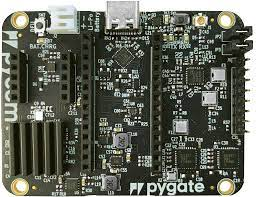
\includegraphics[width=.4\columnwidth]{Pictures/pygate.png}}
\end{wrapfigure}

\lgf{On insère le Pycom sur la Pygate et on connecte l'antenne sur le connecteur du Pygate. Dans un second temps on doit adapter le Pycom à ses nouvelles fonctions, en téléchargeant le bon microprogramme. On le fait en lançant le programme Pycom Firmware Update et en choisissant Pygate. }
\lge{We insert the Pycom on the Pygate and connect the antenna to the Pygate connector. In a second step we need to adapt the Pycom to its new functions, by downloading the right firmware. This is done by launching the Pycom Firmware Update program and choosing Pygate. }


         \vspace{1em}


\lgf{Dans un troisième temps, on ouvre le répertoire Pygate avec Atom. On y trouve le fichier \lprog{wifi\_conf.py}{Pygate} qui va permettre à la Gateway d'avoir accès à votre réseau wifi, il peut contenir les mêmes identifiants que lorsque vous aviez connecter votre LoPY à votre réseau wifi. Le programme \lprog{main.py}{Pygate} est préconfigurée pour utiliser le LNS européen de The Things Network. }
\lge{In a third time, we open the Pygate directory with Atom. We find there the file \lprog{wifi\_conf.py}{Pygate} which is going to allow the Gateway to have access to your wifi network, it can contain the same identifiers as when you had connected your LoPY to your wifi network. The program \lprog{main.py}{Pygate} is preconfigured to use the European LNS of The Things Network. }


         \vspace{1em}

\lgf{Le fichier \lprog{config.json}{Pygate} contient la description des fréquences utilisables dans cette zone. En y jetant un coup d'œil, on peut voir huit fréquences qui sont écoutées par la passerelle radio. Vous trouverez sur le site de The Things Network les autres configurations possibles. }
\lge{The file \lprog{config.json}{Pygate} contains the description of the frequencies that can be used in this area. If you take a look at it, you can see eight frequencies that are listened to by the radio gateway. You can find the other possible configurations on The Things Network website. }


         \vspace{1em}


\lgf{On téléverse le programme dans la mémoire du Pycom de la passerelle radio et comme il s'appelle \lprog{main.py}, il va se lancer tout seul au redémarrage. Il se connecte au wifi, puis va afficher l'identifiant la passerelle. Recopiez le car nous allons avoir besoin plus tard. Après on a plein de texte indiquant que la passerelle est en train de configurer le réseau LoRaWAN. Quand la led passe au vert, la passerelle est active. }
\lge{We download the program in the memory of the Pycom of the radio gateway and as it is called \lprog{main.py}, it will launch itself at reboot. It connects to the wifi, then displays the gateway ID. Copy it because we will need it later. Then we have a lot of text indicating that the gateway is configuring the LoRaWAN network. When the LED turns green, the gateway is active. }

\lgf{\subsection{Configuration de The Things Network}}
\lge{\subsection{Configuration de The Things Network}}


\lgf{Maintenant nous devons informer The Things Networks de l'existence de notre passerelle radio. Si ce n'est pas le cas vous devrez créer un compte sur The Things Network. Aller sur console choisissez \textit{Europe 1} si vous êtes en Europe ou la zone géographique correspondante. Ajoutez une passerelle en donnant : }
\lge{Now we need to inform The Things Networks about the existence of our radio gateway. If not you will have to create an account on The Things Network. Go to console choose \textit{Europe 1} if you are in Europe or the corresponding geographical area. Add a gateway by giving : }


\begin{itemize}
    \item 
        \lgf{un identifiant textuel qui est un non lisible sans espaces~;}
        \lge{a textual identifier which is a non-readable without spaces;}
        
    \item 
        \lgf{l'identifiant de la passerelle qui correspond à la valeur hexadécimale affiché au démarrage~;}
        \lge{the gateway identifier which corresponds to the hexadecimal value displayed at startup;}
        
    \item 
        \lgf{un texte pour mieux décrire la passerelle~;}
        \lge{a text to better describe the gateway;}
        
    \item 
        \lgf{finalement le plan fréquences\footnote{si les objets sont facilement accessibles on peut choisir le Spreading Factor 9 pour la voie descendante sinon si vous n'arrivez pas à joindre vos objets, vous pouvez vous replier sur le Spreading Factor 12}. }
        \lge{finally the frequencies plan{if the objects are easily accessible you can choose the Spreading Factor 9 for the descending path otherwise if you can't join your objects you can fall back on the Spreading Factor 12}. }
        
\end{itemize}

\lgf{On valide la passerelle et elle est ajoutée au LNS. Vous allez pouvoir visualiser les trames qu'elle reçoit.}
\lge{We validate the gateway and it is added to the LNS. You will be able to see the frames it receives.}


\lgf{\section{Vue générale des échanges}}
\lge{\section{General view of the exchanges}}


\lgf{La figure~\vref{fig-ttn-exchanges} en illustre le fonctionnement global. La première émission du LoPy est captée par un ou plusieurs passerelles radio, qui relaient le message via un format JSON spécifique appelé \textit{\Index{Packet Forwarder}}, cela peut être de directement en UDP ou en utilisant MQTT. Le LNS après identification de l'Objet, envoie une requête POST contenant les données émise vers une destination configurée par une URI. Cette requête arrive au routeur du domicile, qui l'envoie à un équipement dans le domicile en fonction de la configuration du NAT. 
Le programme \pprog{generic\_relay.py}{plido-tp3} traite la requête, en extrait le contenu et l'envoie via une socket au programme.
Si ce dernier ne répond pas, le temporisateur se déclenche et la requête est acquitée.}
\lge{The figure~\vref{fig-ttn-exchanges} illustrates the overall operation. The first transmission of the LoPy is picked up by one or more radio gateways, which relay the message via a specific JSON format called \textit{Index{Packet Forwarder}}, this can be directly in UDP or using MQTT. The LNS after identifying the Object, sends a POST request containing the data to a destination configured by a URI. This request arrives at the home router, which sends it to a device in the home depending on the NAT configuration. 
The program \pprog{generic\_relay.py}{plido-tp3} processes the request, extracts its contents and sends it via a socket to the program.
If the latter does not answer, the timer is triggered and the request is acknowledged.}


\lgf{Sinon, si le  programme \pprog{generic\_relay.py}{plido-tp3} reçoit des données en réponse avant le déclenchement du temporisateur, il initie une nouvelle requête POST vers le LNS. Dans notre cote, quand le LNS l'acquitte, la requête initiale est à son tour acquittée. }
\lge{Otherwise, if the program \pprog{generic\_relay.py}{plido-tp3} receives data in response before the timer is triggered, it initiates a new POST request to the LNS. In our example, when the LNS acknowledges it, the initial request is in turn acknowledged. }

\lgf{Le message descendant est gardé en mémoire dans le LNS jusqu'à ce que la fenêtre de réception du Lopy s'ouvre. }
\lgf{The downlinked message is held in memory in the LNS until the Lopy receive window opens. }


\begin{figure}[tbp]

\begin{tikzpicture}

\node[inner sep=0pt] (lopy) at (0,0) {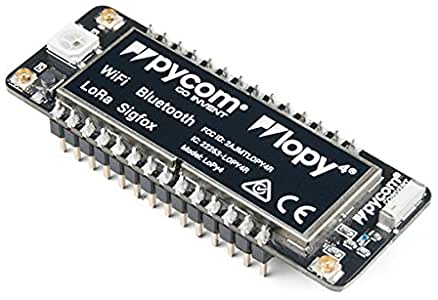
\includegraphics[width=.1\textwidth]{Pictures/LoPy.jpg}};
\node[inner sep=0pt] (RGW) at (3,0) {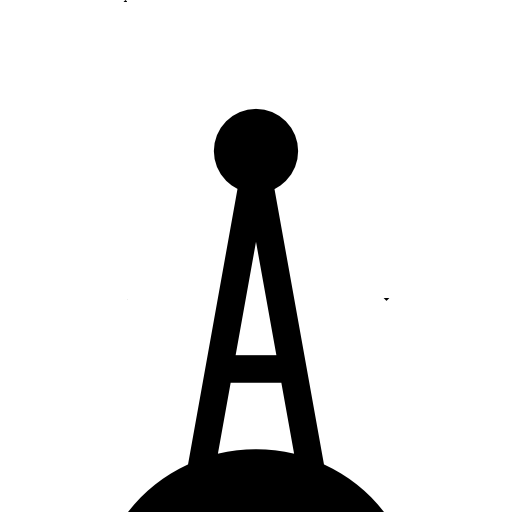
\includegraphics[width=.1\textwidth]{Pictures/antenna.png}};

\draw (5, 0) node (NGW) [cloud, draw] {LNS};

\node[inner sep=0pt] (NAT) at (8,0) {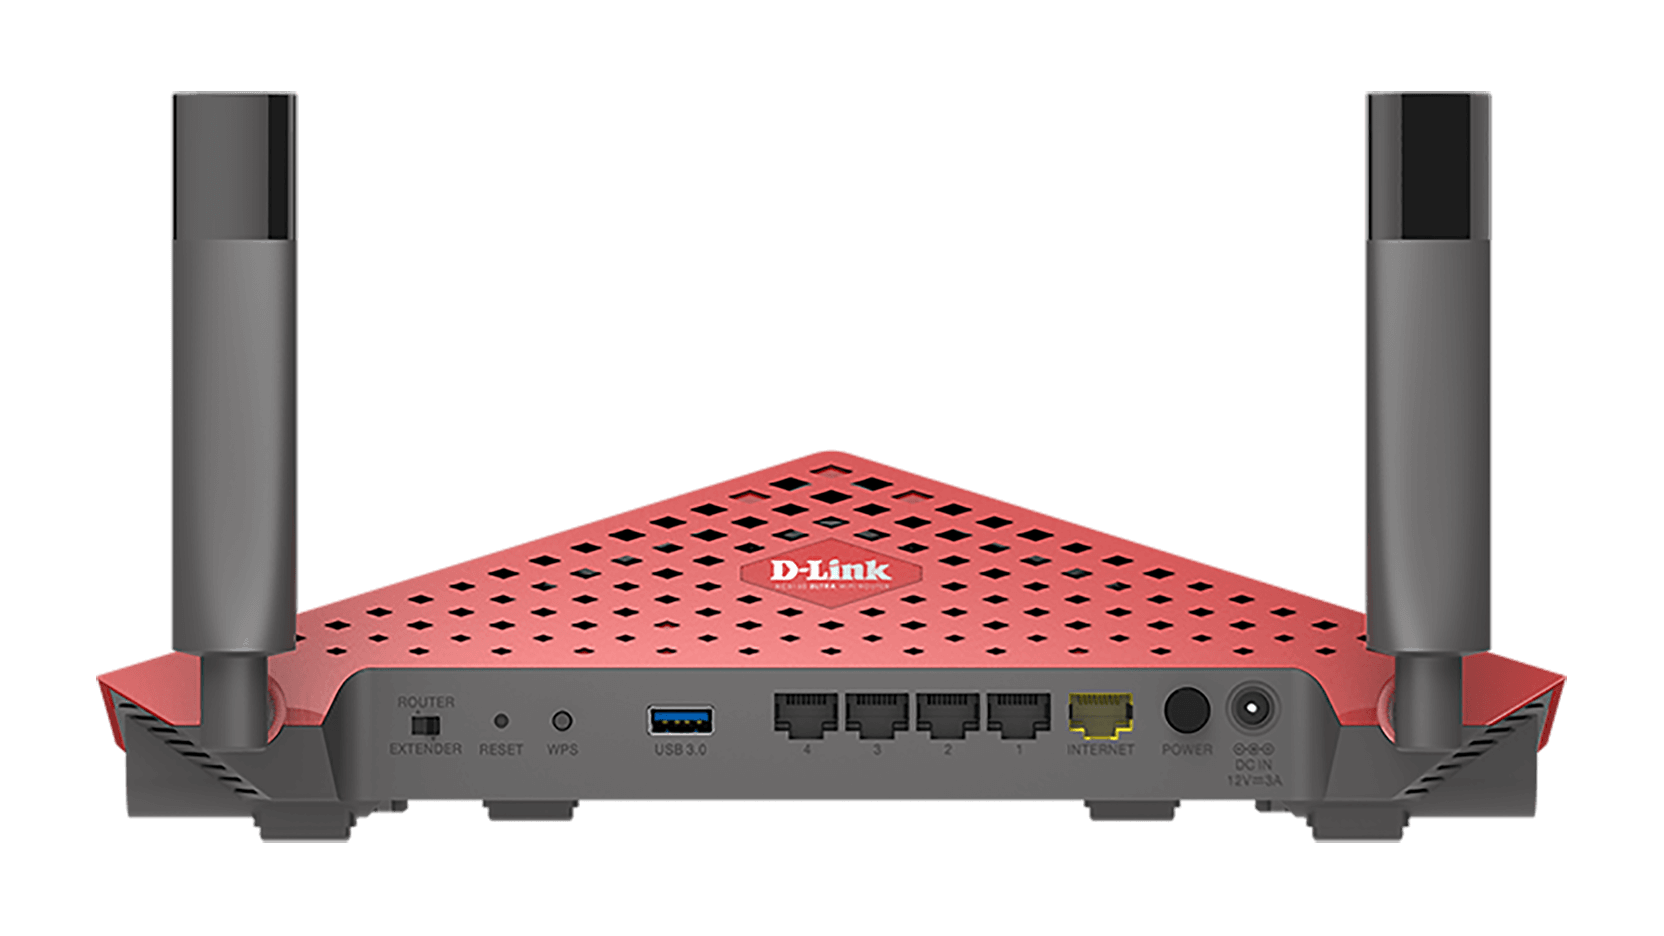
\includegraphics[width=.1\textwidth]{Pictures/router.png}};

\draw (NAT) node [below=15pt] {\small{NAT}};

\draw (12, 0) node (computer) [rectangle, dotted,draw, minimum width=5cm, minimum height=2cm] {};

\draw (10.7, 0) node (relay) [ellipse, dashed, draw, minimum width=2cm, minimum height=1cm] {};
\draw (13.3, 0) node (prog) [ellipse, dashed, draw, minimum width=2cm, minimum height=1cm] {};

\draw (relay) node {\tiny{\texttt{generic\_relay.py}}};
\draw (prog) node {\tiny{\textit{Programme}}};


\draw (12, 0) node [rotate=90] (interface) {\tiny{loopback}};

\draw (computer.north) node [above] {\tiny{Ordinateur}};

\path (lopy) -- +(0, -1.5) coordinate(sline);

\foreach \l in {lopy, RGW, NGW, NAT, relay, prog} {
    \draw [dotted, thin, ->] (\l |- sline) -- +(0, -10); 
}

\path(sline) -- +(0, -0.5) coordinate (a);

\draw (a) node [left, rectangle, draw] {\tiny{msg}};


\draw [decoration={expanding waves,angle=2,segment length=1mm},decorate] (a) -- ([yshift=-0.2cm]a -| RGW) coordinate(b);

\draw [->,decorate,decoration=snake] (b) -- node [above, sloped]{\tiny{packet forwarder}}([yshift=-0.2cm]b -| NGW) coordinate(c); 

\draw [double, double distance=5pt,  green] (c) -- node [above, sloped]{\tiny{POST}} ([yshift=-0.3cm]c -| NAT) coordinate (d); 
\draw [double, double distance=5pt,  orange, ->] (d) --  node [above, sloped]{\tiny{POST}}  ([yshift=-0.3cm]d -| relay) coordinate (e); 
\draw [double, double distance=3pt,  blue] (e) --  node [above, sloped]{\tiny{UDP/IP}}  ([yshift=-0.3cm]e -| prog) coordinate (f); 


\draw (f) node [right, rectangle, draw] {\tiny{msg}};

\draw [thick]  (e) --node [right, near end] {\tiny{Temporisateur}} +(0, -1.5) coordinate (m) ; 

\draw [very thick, orange] (m) -- node [above, sloped]{\tiny{200 OK}}   ([yshift=-0.3cm]m -| NAT) coordinate (n);
\draw [very thick, green, ->] (n) --   node [above, sloped]{\tiny{200 OK}} ([yshift=-0.3cm]n -| NGW) coordinate (o);



% =======
\path(sline) -- +(0, -5) coordinate (a);

\draw (a) node [left, rectangle, draw] {\tiny{msg}};


\draw [decoration={expanding waves,angle=2,segment length=1mm},decorate] (a) -- ([yshift=-0.2cm]a -| RGW) coordinate(b);

\draw [->,decorate,decoration=snake] (b) -- ([yshift=-0.2cm]b -| NGW) coordinate(c); 

\draw [double, double distance=5pt,  green] (c) -- node [above, sloped]{\tiny{POST}} ([yshift=-0.3cm]c -| NAT) coordinate (d); 
\draw [double, double distance=5pt,  orange, ->] (d) --  node [above, sloped]{\tiny{POST}}  ([yshift=-0.3cm]d -| relay) coordinate (e); 
\draw [double, double distance=3pt,  blue] (e) --  node [above, sloped]{\tiny{UDP/IP}}  ([yshift=-0.3cm]e -| prog) coordinate (f); 

\draw (f) node [above right, rectangle, draw] {\tiny{msg}};
\draw (f) node [below right, rectangle, draw] {\tiny{resp}};

\draw [double, double distance=3pt,  blue] (f) --  ([yshift=-0.3cm]f -| relay) coordinate (m); 



\draw [double, double distance=5pt, orange,] (m) -- node [above, sloped]{\tiny{POST}}   ([yshift=-0.3cm]m -| NAT) coordinate (n);
\draw [double, double distance=5pt, green, ->] (n) --   node [above, sloped]{\tiny{POST}} ([yshift=-0.3cm]n -| NGW) coordinate (o);

\draw [thick, -*]  (e) -- (m) coordinate (m) ; 

\draw [very thick, green] (o) --   ([yshift=-0.3cm]o -| NAT) coordinate (s);
\draw [very thick, orange, ->] (s) --   node [above, sloped]{\tiny{200 OK}} ([yshift=-0.3cm]s -| relay) coordinate (t);


\path (t) -- +(0, -0.2) coordinate(w);
\draw [very thick, orange] (w) -- node [above, sloped]{\tiny{200 OK}}   ([yshift=-0.3cm]w -| NAT) coordinate (u);
\draw [very thick, green, ->] (u) --   node [above, sloped]{\tiny{200 OK}} ([yshift=-0.3cm]u -| NGW) coordinate (v);


\draw [dashed, orange] (e) to[bend left] (w);

\path (o) -- +(0, -2) coordinate(p);

\draw [->,decorate,decoration=snake] (p) -- ([yshift=-0.2cm]p -| RGW) coordinate(q); 

\draw [decoration={expanding waves,angle=2,segment length=1mm},decorate] (q) -- ([yshift=-0.2cm]q -| lopy) coordinate(r);

\draw (r) node [left, rectangle, draw] {\tiny{resp}};

\end{tikzpicture}

\lgf{\caption{Diagramme temporel des échanges.}}
\lge{\caption{Time diagram of the exchanges.}}

\label{fig-ttn-exchanges}
\end{figure}

\lgf{\section{Thermomètre LoRaWAN}}
\lge{\section{LoRaWAN Thermometer}}

\lgf{Le programme \lprog{lorawan\_temperature.py}{pycom} combine la manière de rejoindre le réseau LoRaWAN que l'on à vu précédemment et la partie envoie des séries temporelles différentielles des mesures de température. La seule difficulté réside dans la taille de cette série temporelle. En effet, suivant le \Index{Data Rate} le volume de données transportées diffère. Le tableau~\vref{tab-data-rate} donne la correspondance entre le \textit{Data Rate} et les autres paramètres physique. Il indique également la taille maximales des données transportées.}
\lge{The program \lprog{lorawan\_temperature.py}{pycom} combines the way of joining the LoRaWAN network that we have seen previously and the part that sends differential time series of temperature measurements. The only difficulty lies in the size of this time series. Indeed, according to the \Index{Data Rate} the volume of transported data differs. The table~\vref{tab-data-rate} gives the correspondence between the \textit{Data Rate} and the other physical parameters. It also indicates the maximum size of the transported data.}


         \vspace{1em}

\lgf{Ce changement de taille peut poser des problèmes de compatibilités, si l'on choisi une taille trop grande pour être transmise. En théorie, l'on connaît le \textit{Data Rate} choisi et on peut adapter la taille en conséquence, mais l'opérateur peut aussi modifier le \textit{Data Rate} de l'Objet en fonction des conditions de transmission, et il n'existe aucune instruction en micro-python pour récupérer le \textit{Data Rate} réellement utilisé. Pour simplifier la mise en œuvre, la taille maximale de 50 octets a été choisie. }
\lge{This change of size can pose problems of compatibility, if one chooses a size too large to be transmitted. In theory, one knows the \textit{Data Rate} chosen and one can adapt the size consequently, but the operator can also modify the \textit{Data Rate} of the Object according to the conditions of transmission, and there is no instruction in micro-python to recover the \textit{Data Rate} really used. To simplify the implementation, the maximum size of 50 bytes was chosen. }


\begin{table}
\begin{center}
\begin{tabular}{|c||c|c||c|}
\hline
 \rowcolor{purple!10} Data Rate & Spreading Factor & Largeur de bande & Taille Maximum (octets) \\ \hline \hline
 DR0 & SF12 & 125 KHz & 51 \\ \hline
 DR1 & SF11 & 125 KHz & 51 \\ \hline
 DR2 & SF10 & 125 KHz & 51 \\ \hline
 DR3 & SF9 & 125 KHz & 115 \\ \hline
 DR4 & SF8 & 125 KHz & 242 \\ \hline
 DR5 & SF7 & 125 KHz & 242 \\ \hline
 DR6 & SF7 & 250 KHz & 242 \\ \hline
\end{tabular}
\end{center}
\caption{Data Rate en Europe}
\label{tab-data-rate}
\end{table}


\lgf{Il suffit de remplacer \pprog{display\_receive\_and\_send.py}{plido-tp3} par \pprog{display\_server.py}{plido-tp3} pour que la série temporelle soit traitée et le résultat envoyé à Beebotte.}
\lge{Just replace \pprog{display\_receive\_and\_send.py}{plido-tp3} by \pprog{display\_server.py}{plido-tp3} for the time series to be processed and the result sent to Beebotte.}


\Question{US902}
{
\lgf{En vous aidant du lien suivant \url{https://www.thethingsnetwork.org/docs/lorawan/regional-parameters/} indiquant les paramètres régionaux. Est ce que le programme \lprog{lorawan\_temperature.py}{pycom} fonctionnerait sur un réseau LoRaWAN situé en Amérique du Nord~?}
\lge{With the help of the following link \url{https://www.thethingsnetwork.org/docs/lorawan/regional-parameters/} indicating the regional parameters. Would the program \lprog{lorawan\_temperature.py}{pycom} work on a LoRaWAN network located in North America?}

}
{
\lgf{Non, la taille maximale des données pour DR0 est de 11 octets.}
\lge{No, the maximum data size for DR0 is 11 bytes.}
}